\section{Hinweise zur Einleitung}

In der Einleitung sollte das Problem motiviert und begründet werden. Der Umfang des Problems sollte verständlich gemacht werden. Hierfür sollte ein Fließtext verwendet werden. An geeigneten Stellen ist mit Quellen zu arbeiten. Im Text wird die Kurzzitierweise genutzt, wie am Ende dieses Satzes.\footnote{Vgl. \textcite{beispielname2024beispieltitel}, S. 57.} 

Zusätzlich soll bei Abschlussarbeiten eine oder mehrere Forschungsfrage(n) definiert werden. Diese können im Text hervorgehoben werden, z. B. durch 
\begin{center}
    \textit{Hier könnte eine Forschungsfrage stehen. Diese Art der Darstellung eignet sich insbesondere, wenn eine Forschungsfrage präsentiert wird.}
\end{center}
oder durch eine Aufzählung
\begin{itemize}
    \item Hier könnte eine Forschungsfrage stehen.
    \item Hier könnte noch eine Forschungsfrage stehen. Diese Darstellung eignet sich insbesondere bei zwei Forschungsfragen.
\end{itemize}



\section{Beispiele}
\textit{Hier steht in der Arbeit kein Text, da Unterpunkte folgen!}

% Mit \subsection kann ein Unterkapitel erzeugt werden

% ________________________________________________
% Beispiele zum Fließtext
% ________________________________________________
\subsection{Beispiele zum Fließtext}
Der Großteil der schriftlichen Arbeit besteht aus Fließtext. Um Aussagen hervorzuheben, kann es in \underline{\textbf{\textit{Einzelfällen}}} sinnvoll sein, Teile \textbf{fett} oder \textit{kursiv zu} schreiben. Auch das \underline{Unterstreichen von Wörtern} ist möglich. 

An geeigneten Stellen sollten Absätze verwendet werden. Diese lassen sich erzeugen, in dem im Quelltext eine leere Zeile eingefügt wird (wie vor diesem Satz). Durch das Paket \texttt{usepackage[skip=12pt, indent=0pt]{parskip}} wurde in \texttt{preamble.tex} für diese Vorlage festgelegt, dass nach jedem Absatz ein Abstand von 12pt eingefügt wird und der Beginn einer jeden Zeile nicht eingerückt ist. Wenn keine leere Zeile nach einem Absatz gewünscht ist, kann dies dort geändert werden. In jedem Fall ist es sinnvoll, eine gleichbleibende Struktur für die gesamte Arbeit zu wählen.

Wie bei der Einleitung kann mit Quellen in Fußnoten arbeiten, z. B. so.\footnote{Vgl. \textcite{beispielname2024beispieltitel}, S. 1.} Auch Internetseiten lassen sich auf diese Art zitieren.\footnote{\textcite{insitutprod}, \url{https://www.prod.uni-hannover.de/de/lehre/lehrveranstaltungen}} Manchmal gibt es mehrere Quellen zu einer Aussage. Dies können in eine gemeinsame Fußnote aufgenommen werden.\footnote{Vgl. \textcite{beispielname2024beispieltitel}, S. 56-58 und \textcite{beispielname2024beispieltitel2}, S. 7-17.} Ggf. kann es vorkommen, dass eine Quelle direkt im Text genannt wird, wie z. B. bei dem Satz: Das Modell nach \textcite{sudbeck2024using} zeigt \dots.\footnote{Vgl. \textcite{sudbeck2024using}, S. 12-13.} Eine zusätzliche Fußnote kann am Ende des Satzes hinzugefügt werden, um die Seiten anzugeben.

 In Fußnoten können auch Zusatzinformationen oder Anmerkungen untergebracht werden, die beim Lesen des Textes nicht notwendigerweise erforderlich sind.\footnote{Beispielsweise bietet es sich an, bei einer numerischen Untersuchung die genutzte Hardware in einer Fußnote anzugeben.} Für alle Fußnoten gilt, dass diese durch Latex automatisch auf der passenden Seite angezeigt werden.

Anführungszeichen müssen speziell gesetzt werden, wie dieses Beispiel mit "normalen" Anführungszeichen zeigt. Dieses geschieht mit \texttt{glqq} und \texttt{grqq}, wie in diesem Beispiel: \glqq und\grqq. Wenn hinter dem zweiten Anführungszeichen ein weiteres Wort folgt, sodass ein Leerzeichen benötigt wird, muss eine geschweifte Klammer eingefügt werden: Dies ist \glqq ein\grqq{} Beispiel. Ansonsten fehlt das Leerzeichen und das folgende Wort steht direkt am zweiten Anführungszeichen.


% ________________________________________________
% Beispiele zu Abbildungen
% ________________________________________________
\subsection{Beispiele zu Abbildungen}
Eine Abbildung wird wie folgt eingefügt:
    
\begin{figure}
    \centering
    
\includegraphics[width=0.2\textwidth]{Abbildungen/Logo_PROD.png}
    \caption{Logo des Instituts für Produktionswirtschaft}
    \label{fig:Logo_PROD}
\end{figure}


In diesem Fall soll die Grafik bei Breite von 20\% der Textbreite haben. Es können PDFs, PNGs oder JPEGs eingefügt werden. Mit \texttt{caption} wird eine Abbildungsunterschrift eingefügt, welche automatisch ins Abbildungsverzeichnis aufgenommen wird. Um den Arbeitsbereich übersichtlich zu halten, ist es sinnvoll, alle Abbildungen in einem Ordner (in diesem Beispiel \texttt{Abbildungen}) zu sortieren. Über \texttt{label} wird ein Label definiert, sodass auf die Abbildung Bezug genommen werden kann. DIes geschieht dann mit \texttt{autoref}: \autoref{fig:Logo_PROD}.

Latex ordnet Abbildungen (und auch Tabellen) automatisch auf der Seite an. Deshalb erscheint eine Grafik nicht zwingend an der Position, in der sie im Quelltext aufgeführt wurde. \autoref{fig:Logo_PROD} ist ein gutes Beispiel dafür. Soll eine Grafik an einer bestimmten Position platziert werden, so kann dies mit einem \texttt{H} in eckigen Klammern erzwungen werden, wie bei der \autoref{fig:Komponenten_Ladeinfrastruktur}. 

Wird eine Abbildung übernommen, muss die Quelle kenntlich gemacht werden. Damit die Quelle im Abbildungsverzeichnis nicht mit aufgenommen wird und im Dokument einheitlich aufgeführt werden, wurde in \texttt{preamble.tex} der Befehl \texttt{captionsource} definiert. Hiermit kann, wie in \autoref{fig:Komponenten_Ladeinfrastruktur} gezeigt, die Quelle angegeben werden.

\begin{figure}[H]
    \centering
    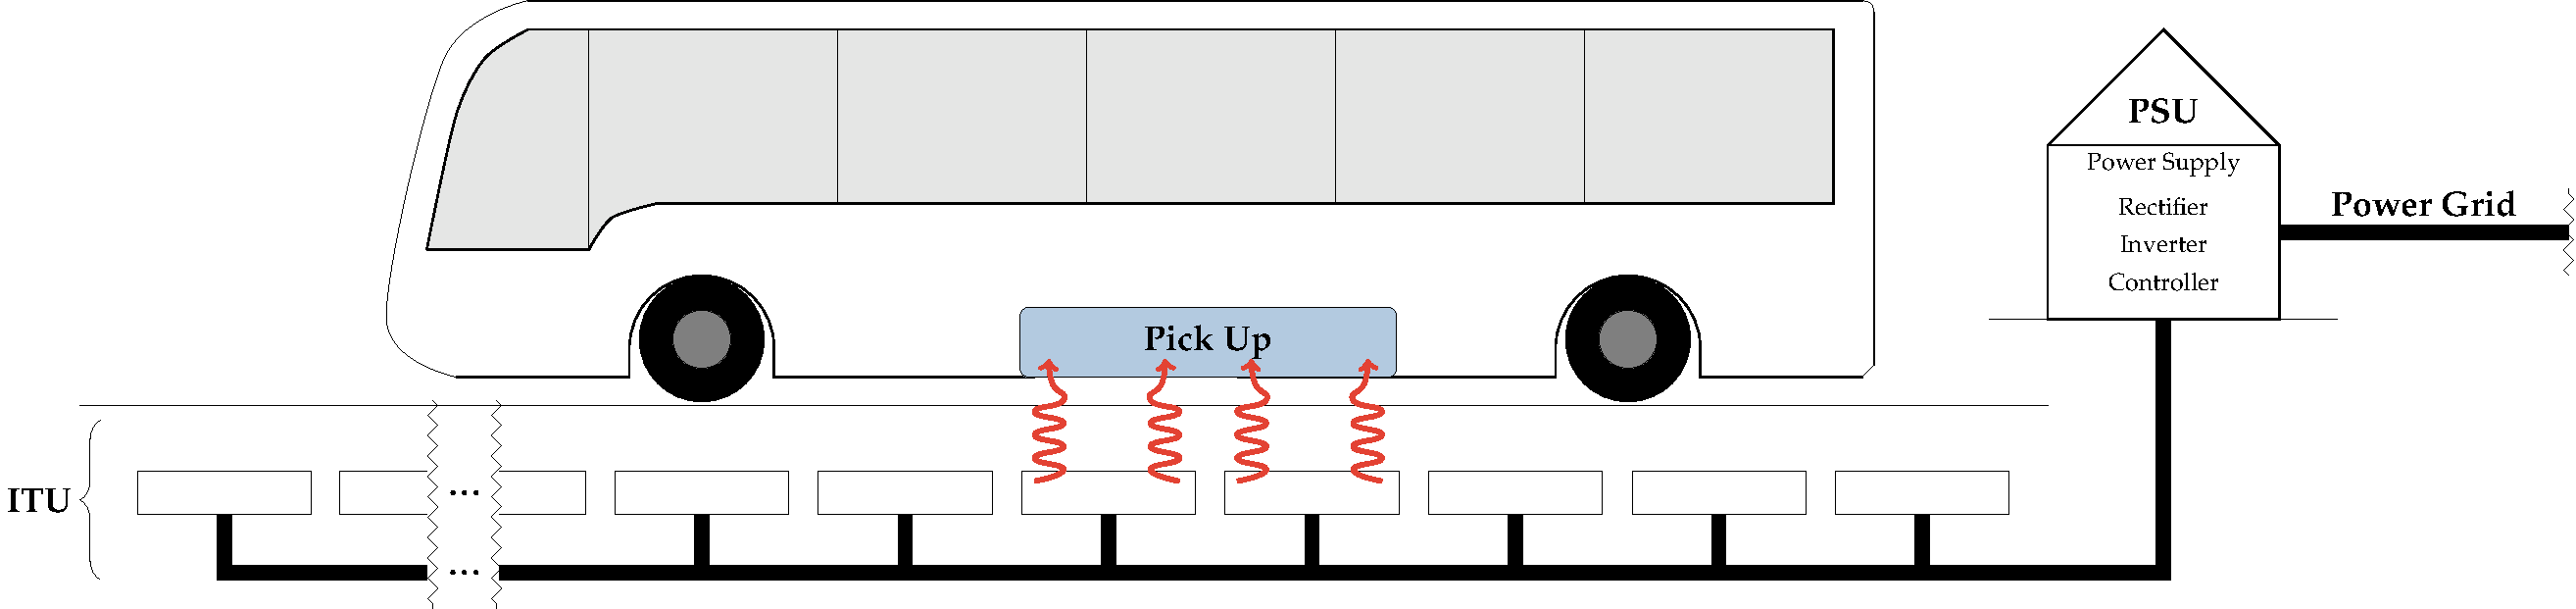
\includegraphics[width=0.9\textwidth]{Abbildungen/Komponenten_dynamisch-induktive_Ladeinfrastruktur.pdf}
    \captionsource{Komponenten einer dynamisch-induktive Ladeinfrastruktur}{\textcite{broihan2022designing}, S. 2}
    \label{fig:Komponenten_Ladeinfrastruktur}
\end{figure}

Ggf. kann es sinnvoll sein, zwei Abbildungen nebeneinander zu platzieren. Es muss aber sichergestellt sein, dass die Abbildungen lesbar bleiben und insbesondere die Schrift hierdurch nicht zu klein wird. Wenn die beiden Abbildungen thematisch eng zusammengehören, eignet sich hierfür eine \texttt{subfigure}, wie in \autoref{fig:Beispiel_Subfigure_gesamt} dargestellt. Diese setzt sich aus \autoref{fig:Beispiel_Subfigure_1} und \autoref{fig:Beispiel_Subfigure_2}. Sollen zwei unabhängige Abbildungen nebeneinander platziert werden, eignet sich die Erstellung einer \texttt{minipage}. Hierbei können dann zwei (oder auch mehrere) Elemente nebeneinander platziert werden, wie bei \autoref{fig:Beispiel_Figure_Minipage_1} und \autoref{fig:Beispiel_Figure_Minipage_2}.

\begin{figure}[H]
    \begin{subfigure}[c]{0.49\textwidth}
        \missingfigure{Hier fehlt die Subfigure links}
        \subcaption{Unterschrift Bild Nr. 1}
        \label{fig:Beispiel_Subfigure_1}
    \end{subfigure}
    \begin{subfigure}[c]{0.49\textwidth}
        \missingfigure{Hier fehlt die Subfigure rechts}
        \subcaption{Unterschrift Bild Nr. 2}
        \label{fig:Beispiel_Subfigure_2}
    \end{subfigure}
    \caption{Zwei Bilder mit Subfigure nebeneinander}
    \label{fig:Beispiel_Subfigure_gesamt}
\end{figure}


\begin{figure}[H]
    \centering
    \begin{minipage}{.5\textwidth}
        \centering
        \missingfigure{Hier fehlt eine Abbildung}
        \captionof{figure}{Hier steht die Unterschrift für die linke Abbildung}
        \label{fig:Beispiel_Figure_Minipage_1}
    \end{minipage}%
    \begin{minipage}{.5\textwidth}
          \centering
          \missingfigure{Und hier fehlt noch eine Abbildung}
          \captionof{figure}{Hier steht die Unterschrift für die rechte Abbildung}
          \label{fig:Beispiel_Figure_Minipage_2}
    \end{minipage}
\end{figure}



% ________________________________________________
% Beispiele zu Tabellen
% ________________________________________________
\subsection{Beispiele zu Tabellen}\label{sec:Tabellen}
Tabellen zu erstellen ist mit Latex leider etwas unübersichtlich, insbesondere wenn diese größer sind. Es gibt allerdings Seiten, mit denen die Tabellen leicht erzeugt und anschließend ins Dokument eingefügt werden können. Ein Beispiel für eine kleine Tabelle ist in \autoref{tab:Beispieltabelle_klein} gegeben. Mit \texttt{lrrr} wird die Ausrichtung der einzelnen Spalten angegeben. Wie bei Abbildungen setzt Latex die Position der Tabellen automatisch, wenn diese nicht festgelegt wurde

\begin{table}
    \centering
    \begin{tabular}{lrrr}
        \toprule
        \textbf{Kategorie} & \textbf{Wert 1} & \textbf{Wert 2} & \textbf{Wert 3} \\ 
        \hline
        A & 10 & 20 & 30 \\ 
        B & 15 & 25 & 35 \\ 
        C & 20 & 30 & 40 \\ 
        D & 25 & 35 & 45 \\ 
        \bottomrule
    \end{tabular}
    \caption{Eine kleine Beispieltabelle}
    \label{tab:Beispieltabelle_klein}
\end{table}

Tabellen können natürlich auch deutlich komplexer gestaltet werden. Beispielsweise ist es möglich, einzelne Zellen miteinander zu verbinden, wie in \autoref{tab:Beispieltabelle_gross} gezeigt. Auch bei Tabellen kann der zuvor definierte Befehl \texttt{captionsource} verwendet werden. 

Um Zahlen mit Einheiten sinnvoll darzustellen, kann das Paket \texttt{numprint} verwendet werden. Mit \np[h]{1.8} wird beispielsweise die Einheit \texttt{h} für Stunde in einem festgelegten Abstand mit der Zahl verbunden. Zusätzlich kann einmalig in \texttt{preamble.tex} eingestellt werden, welche Trennzeichen für Tausender und Dezimalzahlen verwendet werden soll. 

\begin{table}[H]
    \centering
    \begin{tabular}{ll|c|rrr|rrr}
        \toprule
        & & & \multicolumn{3}{c|}{\textbf{Modell 1}} & \multicolumn{3}{c}{\textbf{Modell 2}} \\
        & &\textbf{\# Instanzen} & $\boldsymbol{\overline{t}}$ & $\boldsymbol{\Tilde{t}}$ & $\overline{\text{\textbf{gap}}}$ & $\boldsymbol{\overline{t}}$ & $\boldsymbol{\Tilde{t}}$ & $\overline{\text{\textbf{gap}}}$ \\
        \hline
        \multirow{2}{*}{\textbf{klein}} & \textbf{A} & 20 & \np[s]{3.2} & \np[s]{4.2} & \np[\%]{0} & \np[s]{10.8} & \np[s]{11.9} & \np[\%]{0}\\
        & \textbf{B} & 20 & \np[s]{7.1} & \np[s]{6.9} & \np[\%]{0} & \np[s]{35.2} & \np[s]{40.5} & \np[\%]{0.6} \\
        \hline
        \multirow{2}{*}{\textbf{groß}} & \textbf{A} & 20 & \np[h]{1.2} & \np[h]{1.4} & \np[\%]{0.7} & \np[h]{2} & \np[h]{2} & \np[\%]{5.1} \\
        & \textbf{B} & 20 &  \np[h]{1.8} & \np[h]{2} & \np[\%]{7.3} & \np[h]{2} & \np[h]{2} & \np[\%]{10.8} \\
        \bottomrule
    \end{tabular}
    \captionsource{Eine größere Beispieltabelle}{Hier könnte nun eine Quelle stehen.}
    \label{tab:Beispieltabelle_gross}
\end{table}

% ________________________________________________
% Beispiele zu mathematischen Formeln, Notation und Modellannahmen
% ________________________________________________
\subsection{Beispiele zu mathematischen Formeln, Notation und Modellannahmen}
Wie Zahlen mit Einheiten geschrieben werden können, wurde in \autoref{sec:Tabellen} gezeigt.\footnote{Hier zeigt sich, dass man auch ein Kapitel mit einem \texttt{label} versehen kann und darauf verwiesen werden kann.}

Um mathematische Formeln im Text darzustellen, wird das \$-Zeichen verwendet. So kann zum Beispiel die Variable $x_i$ einfach im Text genannt werden. Auch ein Variable mit zwei Indizes ist möglich, hier müssen allerdings geschweifte Klammern verwendet werden $y_{ij}$. Analog dazu kann man Variable mit hochgestelltem Index haben: $c_i^{g}$.

Längere Formeln sollten nicht im Fließtext stehen, sondern abgesetzt werden, wie bei
\begin{equation} 
    \rho=\frac{\lambda}{\mu}.
\end{equation}

Vergibt man bei einer Formel ein \texttt{label}, so kann man im späteren Text darauf Bezug nehmen, z. B.
\begin{equation}
   E[W_q] \approx \frac{c_a^2+c_s^2}{2} \cdot \frac{\rho}{1-\rho}\cdot \frac{1}{\mu}.\label{eq:Kingmansche_aprrox}
\end{equation}

Nun lässt sich im Text Bezug darauf nehmen. Auch hier kann \texttt{autoref} verwendet werden, dies sieht dann so aus: \autoref{eq:Kingmansche_aprrox}. Hierbei werden die runden Klammern jedoch nicht mit ausgegeben. Daher wurde ein eigener Befehl in \texttt{preamble.tex} erstellt. Mit \texttt{myeqref} wird die Gleichung nun mit runden Klammern dargestellt: \myeqref{eq:Kingmansche_aprrox}.

Einige mathematische Zeichen können direkt von der Tastatur verwendet werden, wie z. B. das Plus: $+$. Andere, wie beispielsweise beim Multiplikationszeichen ($\cdot$), haben spezielle Befehle. Auch griechische Buchstaben lassen sich einfach darstellen, wie z. B. $\alpha$.

Sind Gleichungen zu lang für eine Zeile, lassen sich diese mit über mehrere Zeilen darstellen, wie in \myeqref{eq:Erwartungswert_Fehlmenge}.

\begin{equation}
\begin{aligned}
    E[F(q)] &= \sum_{d=0}^{\infty} \max(d-q,\; 0) \cdot \text{Prob}[D=d] \\
    & = \sum_{d=q}^{\infty} (d-q) \cdot \text{Prob}[D=d]
    \label{eq:Erwartungswert_Fehlmenge}
\end{aligned}
\end{equation}


Auch mathematische Optimierungsmodelle lassen sich mithilfe dieser Art darstellen. Bevor ein Modell eingeführt wird, muss jedoch die Notation \underline{ausführlich} eingeführt werden (Dies bedeutet, dass die Notation \textbf{nicht} nur in einer Tabelle eingeführt wird!). 

Notation lässt sich im Fließtext beschreiben, z. B.:  Im Modell der Ablaufplanung bezeichnet $j \in \mathcal{J} = \{1, ..., J\}$ die Menge der Jobs und $r \in \mathcal{R} = \{1, ..., R\} $ die Menge der Ressourcen. Weiterhin stellt $t,\tau \in \mathcal{T} = \{1, ..., T\}$ die Perioden da mit $T$ als letzte Periode. Für jeden Job $j$ gibt es bestimmte durchzuführende Prozessschritte, welche durch die Menge $s \in \mathcal{S}_j = \{1, ..., ls_j\}$ beschrieben werden. Der letzten Prozessschritt von Job $j$ ist definiert als $ls_j$. Die Durchführung des Prozessschritts $s$ von einem Job $j$ erfordert zu jedem Zeitpunkt $a_{jsr}$ Kapazitätseinheiten der Ressource $r$. \dots

Alternativ ist es auch möglich, die Notation als Aufzählung (in jeweils vollständigen Sätzen) einzuführen, z. B.:
\begin{itemize}
    \item Im Modell der Ablaufplanung bezeichnet $j \in \mathcal{J} = \{1, ..., J\}$ die Menge der Jobs und $r \in \mathcal{R} = \{1, ..., R\} $ die Menge der Ressourcen. 
    \item Die Perioden werden mit der Menge $t,\tau \in \mathcal{T} = \{1, ..., T\}$ beschrieben mit $T$ als letzte Periode. 
    \item Für jeden Job $j$ gibt es bestimmte durchzuführende Prozessschritte, welche durch die Menge $s \in \mathcal{S}_j  = \{1, ..., ls_j\}$ beschrieben werden. Hierbei bezeichnet $ls_j$ den letzten Schritt von Job $j$.
    \item Die Durchführung des Prozessschritts $s$ von einem Job $j$ erfordert zu jedem Zeitpunkt $a_{jsr}$ Kapazitätseinheiten der Ressource $r$.
    \item \dots
\end{itemize}

Bitte denken Sie daran, dass auch die \textbf{Entscheidungsvariablen} zur Notation gehören und \textbf{erläutert} werden müssen!

Zusätzlich ist es bei Abschlussarbeiten sinnvoll, die Notation in einer Tabelle übersichtlich zusammenzufassen (vgl. \autoref{tab:Notation_Ablaufplanung}).

\begin{table}
    \centering
    \caption{Notation zum Modell der Ablaufplanung}
    \label{tab:Notation_Ablaufplanung}
    \begin{tabular}{l p{11cm}}
        \hline
        \multicolumn{2}{l}{\textbf{Indizes und Mengen}} \\
        \hline
        $j \in \mathcal{J} = \{1, ..., J\} $  & Jobs   \\
		$r \in \mathcal{R} = \{1, ..., R\} $  & Ressourcen  \\
		$s \in \mathcal{S}_j = \{1, ..., ls_j\}$ & Schritte des Jobs $j$ \\
		$t, \tau \in \mathcal{T} = \{1, ..., T\}$ & Perioden \\
        \hline
        \multicolumn{2}{l}{\textbf{Parameter}} \\
        \hline
        $a_{jsr}$ & benötigte Kapazitätseinheiten der Ressource $r$ für Schritt $s$ des Jobs $j$\\
        $b_{r t}$ & Kapazität der Ressource $r$ in Periode $t$ \\
        \dots \\
        \hline
        \multicolumn{2}{l}{\textbf{Entscheidungsvariablen}} \\
        \hline
        $X_{jst}^{tP} \in \{0,1\}$ & binäre Variable mit Wert 1, wenn in Periode $t$ der Schritt $s$ des Jobs $j$ beendet wird und 0 sonst\\
        \dots \\
        \bottomrule
    \end{tabular}
\end{table}

Nach der Einführung der Notation kann das Modell eingeführt werden.

\begin{equation}
\textrm{min} \  Z = c \cdot \sum_{j \in \mathcal{J}} TF_{j, ls_j} \label{eq:Ablauf_Zielfunktion}
\end{equation}
\vspace{-24pt} %Verringert den Abstand an der Stelle
\begin{flalign}
\noalign{unter Beachtung der Restriktionen}
\hspace{1cm}& \sum_{t=1}^{T} X_{j s t} = 1 &\forall j \in \mathcal{J},  s \in \mathcal{S}_j \label{eq:Ablauf_Schritte_einmal_beenden}\\ 
%
& TF_{j s} \geq TF_{j, s-1} + d_{j s} & \forall j \in \mathcal{J}, s \in \{2, ..., ls_j\} \label{eq:Ablauf_Schritte_Reihenfolge}\\
%
& \sum_{t=1}^{T} t \cdot X_{j s t} = TF_{j s} & \forall j \in \mathcal{J}, s \in \mathcal{S}_j \label{eq:Ablauf_Kopplung_X_TF}  \\ 
%
& \sum_{j \in \mathcal{J}}\sum_{s \in \mathcal{S}_j}\sum_{\tau=t}^{t + d_{j s} - 1} a_{j s r} \cdot X_{j s \tau} \leq b_{r t} & \forall r \in \mathcal{R}, t \in \mathcal{T} \label{eq:Abl0auf_Kapazitaet}
\end{flalign}
Auf die einzelnen Restriktionen kann nun Bezug genommen werden. Da es sich hierbei um Restriktionen handelt, sollte das Wort \glqq Restriktion\grqq{} genutzt werden. Damit die Referenzierung richtig funktioniert, gibt es auch hierfür in \texttt{preamble.tex} den selbst definierten Befehl \texttt{myrestref}.
Somit können wir beschreiben, dass durch \myrestref{eq:Ablauf_Schritte_einmal_beenden} jeder Schritt in einem Job in genau einer Periode beendet wird und \myeqref{eq:Abl0auf_Kapazitaet} die Zielfunktion darstellt, in welcher \dots.

% ________________________________________________
% Beispiel zu Pseudocode
% ________________________________________________
\subsection{Beispiel zu Pseudocode}
Bei Algorithmen ist es sinnvoll, diese als Pseudocode in der Arbeit zu veranschaulichen. Der eigentliche Code wird im Anhang der Arbeit aufgeführt (vgl. \autoref{sec:Python_Bsp}). Für Pseudocode gibt es eigene Pakete in Latex (\texttt{algorithm} und \texttt{algorithmic}). Ein Beispiel für einen Pseudocode ist in \autoref{alg:Heuristik_TSP} gegeben.

\begin{algorithm}[H]
	\caption{Nearest Neighbor-Heuristik für das TSP - Hauptroutine}
    \label{alg:Heuristik_TSP}
    \begin{algorithmic}[1]
		\WHILE{$Unvisited \neq \emptyset$}
    		\STATE{$dist_{min} = \infty$}
    		\STATE{$i = NextTown$}
    		\FOR{$j \in Unvisited$}
        		\IF{$d(i,j) < dist_{min}$}
            		\STATE{$dist_{min} = d(i,j)$}
            		\STATE{$NextTown = j$}
        		\ENDIF
    		\ENDFOR
    		\STATE{$dist_{tot} = dist_{tot} + dist_{min}$}
    		\STATE{$Unvisited = Unvisited - NextTown$}
    		\STATE{$Tour = Tour + NextTown$}
		\ENDWHILE
		\STATE{$dist_{tot} = dist_{tot} + d(j,s)$}
	\end{algorithmic}
\end{algorithm}

% ________________________________________________
% Beispiel zu To-dos
% ________________________________________________
\subsection{Beispiel zu To-dos}
Mit dem Paket \texttt{todonotes} lassen sich in der Arbeit Kommentare/To-dos einfügen. Diese können entweder im Text stehen:
\todo[inline]{Hier steht eine Aufgabe, die noch gemacht werden muss.}

oder auch an den Seitenrand \todo{z. B.: Hier muss noch eine Quelle gesucht werden.} geschrieben werden.

Zu Beginn der Arbeit kann auch eine Übersicht mit allen To-dos ausgegeben werden (siehe \texttt{listoftodos} in \texttt{main.tex}). Diese Übersicht sollte natürlich \textbf{vor Abgabe der Arbeit auskommentiert} werden. Auch Platzhalter für Abbildungen, die mit \texttt{missing\-figure} erstellt wurden (vgl. \autoref{fig:Beispiel_Figure_Minipage_1}), werden in die Übersicht mit aufgenommen.

% ________________________________________________
% Beispiele zu Farben
% ________________________________________________
\subsection{Beispiele zu Farben}
Farben können eingesetzt werden, um Aspekte gezielt zu betonen oder um Abbildungen gut erkennbar zu machen. Gleichzeitig sollten Farben in einer wissenschaftlichen Arbeit \textbf{sparsam} eingesetzt werden. Mit dem Paket \texttt{xcolor} und der Option \texttt{dvipsnames} (siehe \texttt{preamble.tex}) stehen 68 vordefinierte Farben zur Verfügung. Alternativ können in \texttt{preamble.tex} auch eigene Farben definieren werden, wie dies in dieser Vorlage mit den Farben der Leibniz Universität gemacht wurde. Es empfiehlt sich, im Rahmen der Arbeit einige wenige, zueinander passende Farben auszuwählen und diese in der Arbeit durchgängig einzusetzen. 

Mit einer Farbe können beispielsweise \textcolor{luhblau}{Textabschnitte eingefärbt} werden. Auch lässt sich ein Text \colorbox{luhgruen}{farbig unterlegen}. Auch Aufzählungen lassen sich einfärben:
\begin{itemize}
    \color{luhmittelblau}
    \item Erster Punkt
    \item Zweiter Punkt
\end{itemize}

Insgesamt stellt eine farbige Markierung von Text in einer wissenschaftlichen Arbeit aber die Ausnahme da. Auch in Abbildungen lassen sich die Farben dann verwenden (vgl. \autoref{fig:Abbildung_Farben}).

\begin{figure}[H]
    \centering
    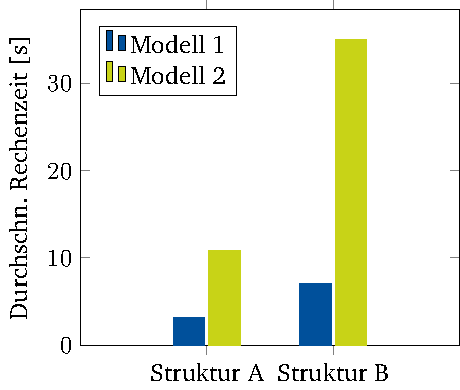
\includegraphics[width=0.5\textwidth]{Abbildungen/Bsp_Abb_Farben_1.pdf}
    \caption{Farben in Abbildungen}
    \label{fig:Abbildung_Farben}
\end{figure}

% ________________________________________________
% Beispiel zu TikZ
% ________________________________________________
\subsection{Beispiele zu TikZ}

Mit dem Paket \texttt{tikz} lassen sich auch andere Abbildungen direkt in Latex erstellen. Dies ist jedoch fortgeschritten und wird, insbesondere bei Bachelor- und Seminararbeiten, nicht von Ihnen erwartet. Wer interessiert ist, kann sich natürlich aber trotzdem die folgenden Beispiele anschauen, welche in \autoref{fig:tikz_graph} und \autoref{fig:tikz_zeichnung} dargestellt sind. Zu Tikz Grafiken findet sich vieles im Internet und auch KI-Tools wie ChatGPT lassen sich gut nutzen, um diese Grafiken zu erstellen.


\begin{figure}[H]
    \centering
    % Set global arrow style
\tikzset{>=Stealth}

% Zeichnung des Windrads, sodass dieses mehrmals verwendet werden kann
\tikzset{%
	wind turbine/.pic={
		\tikzset{path/.style={fill, draw=white, ultra thick, line join=round}}
		\path [path] 
		(-.25,0) arc (180:360:.25 and .0625) -- (.0625,3) -- (-.0625,3) -- cycle;
		\foreach \i in {90, 210, 330}{
			\ifcase#1
			\or
			\path [path, shift=(90:3), rotate=\i] 
			(.5,-.1875) arc (270:90:.5 and .1875) arc (90:-90:1.5 and .1875);
			\or
			\path [path, shift=(90:3), rotate=\i] 
			(0,0.125) -- (2,0.125) -- (2,0) -- (0.5,-0.375) -- cycle;
			\or
			\path [path, shift=(90:3), rotate=\i]
			(0,-0.125) arc (180:0:1 and 0.125) -- ++(0,0.125) arc (0:180:1 and 0.25) -- cycle;
			\fi
		}
		\path [path] (0,3) circle [radius=.25];
}}


\resizebox{0.9\linewidth}{!}{%
	\begin{tikzpicture}[
		task/.style={circle, draw=black, thick, minimum size=12mm, inner sep=0pt, font=\Large},
		teams/.style={rectangle, fill=black!6, draw=black, anchor=west, thick, minimum height=1cm, minimum width=5cm, inner sep=0pt, font=\Large, text width =4.8cm},
		dach/.style={isosceles triangle, draw, inner sep=0pt,
			anchor=south, shape border rotate=90, isosceles triangle stretches, minimum width=5cm, minimum height=1cm},
		body/.style={trapezium, draw, minimum width=0.4cm, minimum height=0.4cm, trapezium stretches},
		head_1/.style={circle, draw, minimum size=0.2cm, fill=luhgruen},
		head_2/.style={circle, draw, minimum size=0.2cm, fill=luhblau}
		]
		
		% House Team 1
		\node[teams, label={[anchor=west, inner sep=0pt, xshift=0.1cm]west:Team-Typ $m1$}] (team_1) at (2, 2) {};
		\node[dach] (dach_team_1) [above = 0cm of team_1] {};
		\node[body] (body_per_1) [below right = 0.5cm and 1.4cm of dach_team_1] {};
		\node[head_1] (head_per_1) [below right = 0.25cm and 1.41cm of dach_team_1] {};
		\node[body] (body_per_2) [below right = 0.5cm and 0.6cm of dach_team_1] {};
		\node[head_1] (head_per_2) [below right = 0.25cm and 0.61cm of dach_team_1] {};
		\node[body] (body_per_3) [below right = 0.5cm and -0.2cm of dach_team_1] {};
		\node[head_1] (head_per_3) [below right = 0.25cm and -0.19cm of dach_team_1] {};
		
		% House Team 2
		\node[teams, label={[anchor=west, inner sep=0pt, xshift=0.1cm]west:Team-Typ $m2$}] (team_2) [right = 8cm of team_1] {};
		\node[dach] (dach_team_2) [above = 0cm of team_2] {};
		\node[body] (body_per_4) [below right = 0.5cm and 1.4cm of dach_team_2] {};
		\node[head_2] (head_per_4) [below right = 0.25cm and 1.41cm of dach_team_2] {};
		\node[body] (body_per_5) [below right = 0.5cm and 0.6cm of dach_team_2] {};
		\node[head_2] (head_per_5) [below right = 0.25cm and 0.61cm of dach_team_2] {};
		\node[body] (body_per_6) [below right = 0.5cm and -0.2cm of dach_team_2] {};
		\node[head_2] (head_per_6) [below right = 0.25cm and -0.19cm of dach_team_2] {};
		
		% Task with turbine
		\node[task] (task_1) [above right = 4cm and -1cm of team_1] {$i1$};
		\path (5.3, 6.4) pic[scale=0.3] {wind turbine=1};
		\node[task] (task_2) [above right = 2.5cm and -3.5cm of team_1] {$i2$};
		\path (3.1,4.1) pic[scale=0.3] {wind turbine=1};
		\node[task] (task_3) [above right = 4cm and 8.5cm of team_1] {$i3$};
		\path (17.2,6.4) pic[scale=0.3] {wind turbine=1};
		\node[task] (task_4) [above right = 0.5cm and 3.5cm of team_1] {$i4$};
		\path (12,2.3) pic[scale=0.3] {wind turbine=1};
		\node[task] (task_5) [above right = -1cm and 2.5cm of team_1] {$i5$};
		\path (11.2,1.3) pic[scale=0.3] {wind turbine=1};
		
		% Arrows Team 1
		\draw [luhgruen, ultra thick, ->] (dach_team_1.north) -- node [pos=0.15,above,color=black] {$z1$} (task_3.west);
		\draw [luhgruen, ultra thick, ->] (task_3.south) -- (dach_team_1);
		
		\draw [luhgruen, ultra thick, ->] (dach_team_1) -- node [pos=0.6, below,color=black] {$z2$} (task_4);
		\draw [luhgruen, ultra thick, ->] (task_4) -- (task_5);
		\draw [luhgruen, ultra thick, ->] (task_5) -- (dach_team_1);
		
		% Arrows Team 2
		\draw [luhblau, ultra thick, ->] (dach_team_2.north) -- node [pos=0.25,above,color=black] {$z1$} (task_1);
		\draw [luhblau, ultra thick, ->] (task_1) -- (task_2);
		\draw [luhblau, ultra thick, ->] (task_2) -- (dach_team_2);
		
	\end{tikzpicture}
}

    \caption[Dies ist ein Beispiel für eine Abbildung mit TikZ.]{{Dies ist ein Beispiel für ein Diagramm mit TikZ.\\{\small Tipp: Auch hierbei die zuvor definierten Farben nutzen.}}}
    \label{fig:tikz_graph}
\end{figure}



\begin{figure}[H]
    \centering
    \begin{tikzpicture}

    % Koordinaten der Orte
    \coordinate (Depot) at (0, 0);
    \coordinate (Ort1) at (2, 2);
    \coordinate (Ort2) at (4, 0);
    \coordinate (Ort3) at (2, -2);
    \coordinate (Ort4) at (-2, -2);
    \coordinate (Ort5) at (-4, 0);
    \coordinate (Ort6) at (-2, 2);
    \coordinate (Ort7) at (1, 3);
    \coordinate (Ort8) at (-1, 3);
    
    % Depot
    \node[draw, circle, luhblau] (D) at (Depot) {D};
    
    % Orte und Kapazitäten
    \node[draw, circle] (1) at (Ort1) {1};
    \node[draw=none, font=\small] at (2.5, 2.5) {4};
    
    \node[draw, circle] (2) at (Ort2) {2};
    \node[draw=none, font=\small] at (4.5, 0.5) {2};
    
    \node[draw, circle] (3) at (Ort3) {3};
    \node[draw=none, font=\small] at (1.5, -2.5) {3};
    
    \node[draw, circle] (4) at (Ort4) {4};
    \node[draw=none, font=\small] at (-2.5, -2.5) {1};
    
    \node[draw, circle] (5) at (Ort5) {5};
    \node[draw=none, font=\small] at (-4.5, -0.5) {5};
    
    \node[draw, circle] (6) at (Ort6) {6};
    \node[draw=none, font=\small] at (-2.5, 2.5) {3};
    
    \node[draw, circle] (7) at (1, 3) {7};
    \node[draw=none, font=\small] at (0.5, 3.5) {2};
    
    \node[draw, circle] (8) at (-1, 3) {8};
    \node[draw=none, font=\small] at (-1.5, 3.5) {4};
    
    % Touren
    \draw[->] (D) -- (1);
    \draw[->] (1) -- (2);
    \draw[->] (2) -- (3);
    \draw[->] (3) -- (D);
    
    \draw[->] (D) -- (4);
    \draw[->] (4) -- (5);
    \draw[->] (5) -- (6);
    \draw[->] (6) -- (D);
    
    \draw[->] (D) -- (7);
    \draw[->] (7) -- (8);
    \draw[->] (8) -- (D);

\end{tikzpicture}
    \caption{Dies ist ein weiteres Beispiel für eine Abbildung mit TikZ.}
    \label{fig:tikz_zeichnung}
\end{figure}

